\SACCMD{benioff}
\label{cmd:benioff}

\SACTitle{概要}
对数据使用Benioff滤波器

\SACTitle{语法}
\begin{SACSTX}
BENIOFF
\end{SACSTX}

\SACTitle{说明}
1960年左右,美国空军VELA计划中使用了一些可变磁阻短周期地震仪,这些仪器以
加州理工的Hugo Benioff教授命名。其自然频率为 \SI{1}{\Hz},与一个电流计
耦合在一起(自然频率为 \SI{5}{\Hz})。耦合因子的标称值为0.01,其响应在
\SI{1}{\Hz} 到 \SI{5}{\Hz} 频段内近乎为平的。

该命令生成的滤波器是Benioff短周期地震仪的数字等效,用于将宽频带地震数据
模拟成短周期系统。

该滤波器的响应函数如下图所示:

\begin{figure}[H]
\centering
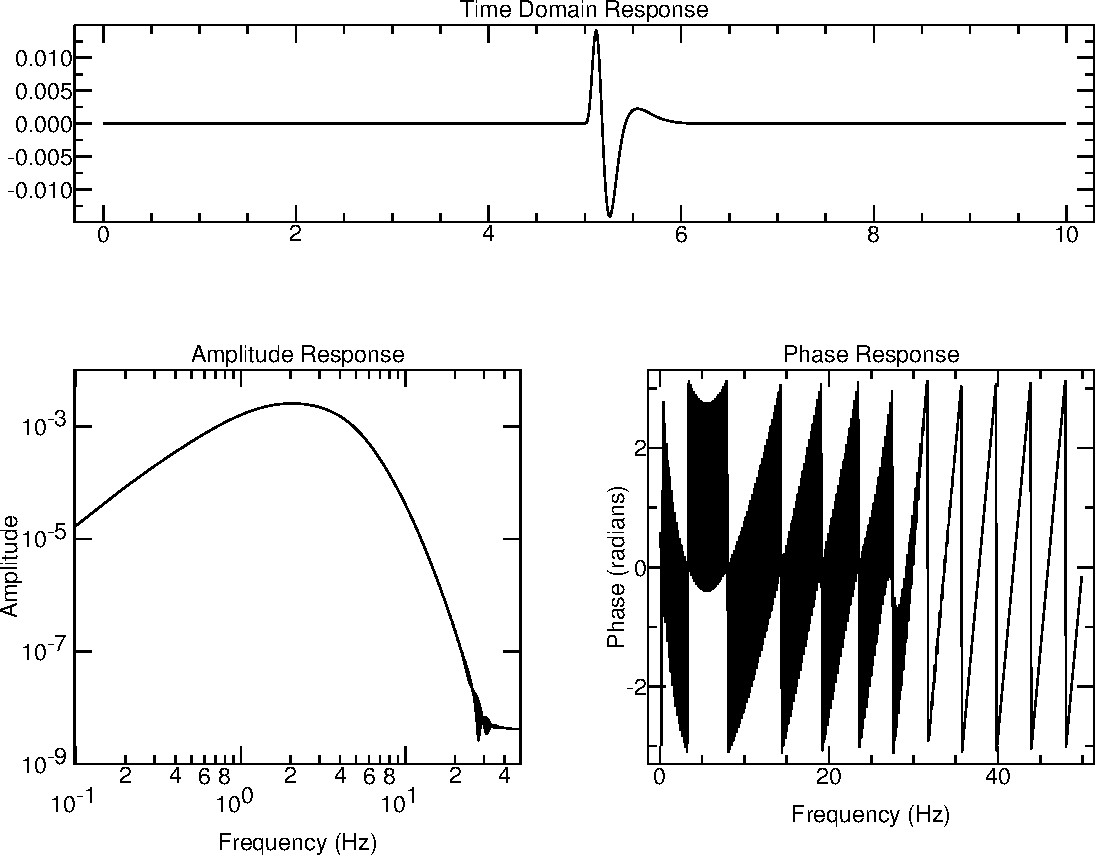
\includegraphics[width=0.8\textwidth]{benioff}
\caption{Benioff滤波器的响应函数}
\label{fig:benioff}
\end{figure}

\SACTitle{头段变量}
depmin、depmax、depmen
